%Discuss how development processed, problems encountered and how some features were cut or added.
\chapter{Development Process}
Work schedule during 13 week period.\\
during 3 week period.

\section{Timeplan}%Cebrail/Jonathan
There are several time planning models in the software world. There is agile, iterative and incremental.
\newline
When we started the `Fagprojekt' we created a waterfall chart containing our plans for every week, it was structured in a waterfall chart. The waterfall chart is a sequential design process. It is designed to get through the project phases and have a product as soon as possible. The phases in our project can be seen in the figure below.
\newline
As we revisited our waterfall model steps over time, our main time plan model can be considered to be iterative. The revisits have mainly been to extend features,debugging or optimizing.
\newline
When the waterfall ends and we still have time
we will go back and visit the steps and check for new requirements.
\newline
The waterfall gives a good picture of the big phases, but the pre-planned week schedules are not always much help, as they are not dynamic. We can't reconstruct our waterfall every time we meet a conflict. This is here where the timeboxes are handy, which is used to the most detailed part of the time planning - see next subsection. You can check our waterfall timeplan in the appendices, please see Figure~\ref{fig:Waterfall_chart} for that.
\begin{figure}[h]
\centering
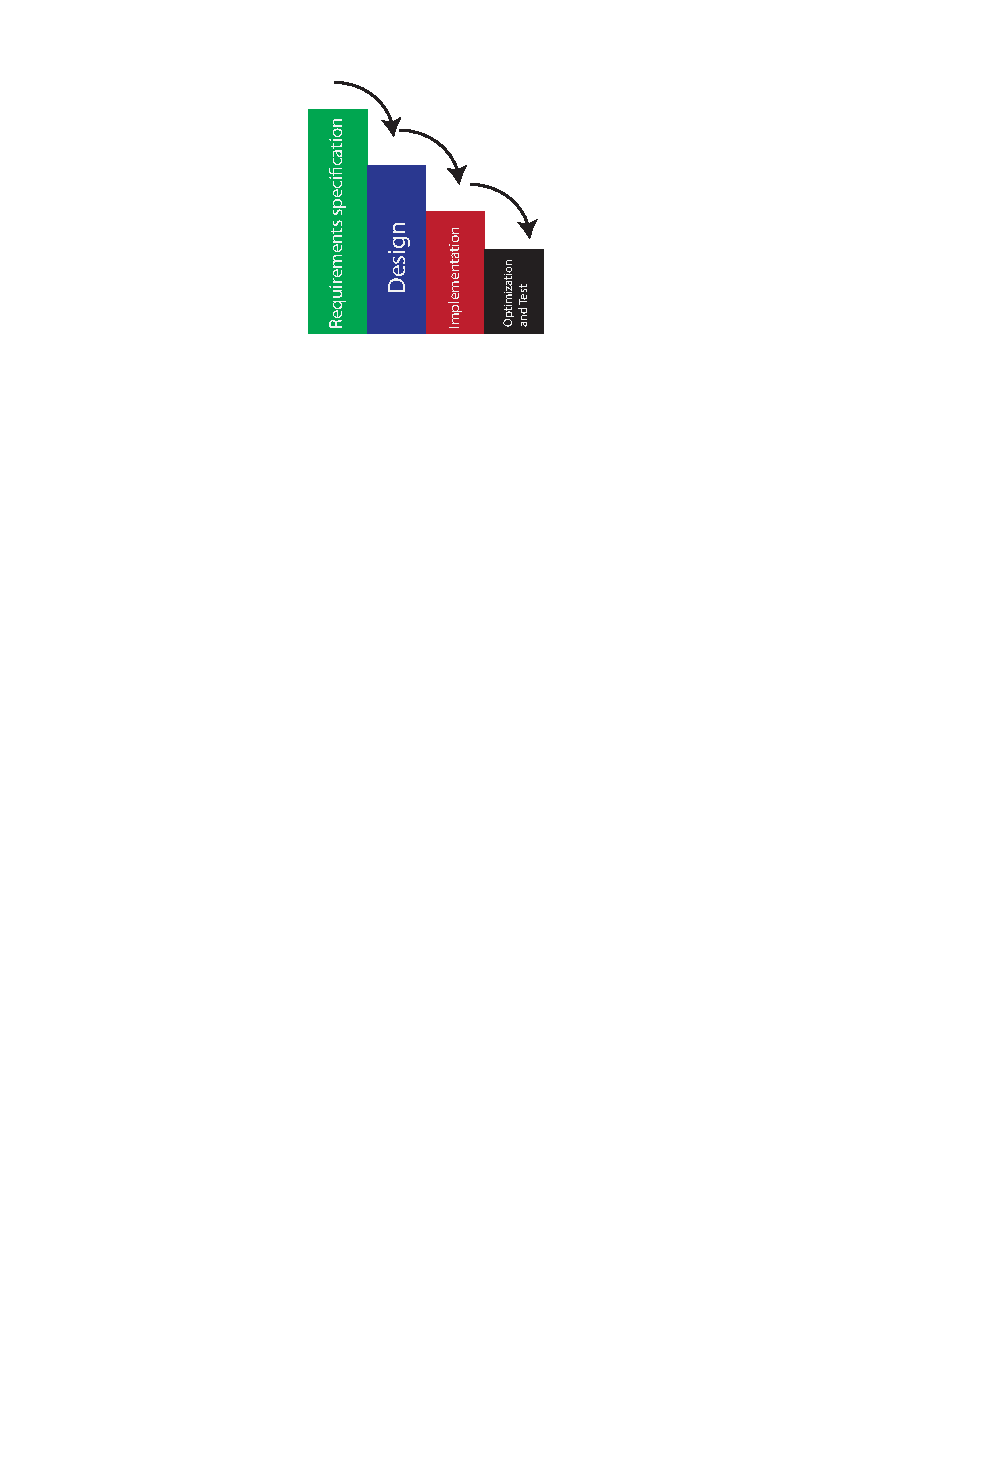
\includegraphics[scale=0.6]{Figures/Waterfall}
\caption{An overview of the waterfall phases.}
\label{fig:Waterfall}
\end{figure}
\newpage

\subsection{Time Boxing} %Jonathan
We were convinced that using "Time Boxing" would be the way to go. Timeboxing divides The schedule into a number of separate time periods(timeboxes), with each part having its own deliverables, deadline and budget. Breaking bigger tasks into smaller tasks with better manageable time frames. What also is important is that by the end of each timebox we need to have a product that if all else fails we can roll back and release our game from an earlier state. The following table shows the timeboxes we have created during the project.
%Please add the following required packages to your document preamble:
%\usepackage[table,xcdraw]{xcolor}
%If you use beamer only pass "xcolor=table" option, i.e. \documentclass[xcolor=table]{beamer}
\begin{table}[h]
\begin{tabular}{llll}
  \rowcolor[HTML]{BBDAFF}
  \textbf{week 8-10}	& \textbf{week 11-13}	& \textbf{week 14-15}	& \textbf{week 16-17}	\\
  Code exercise			& Collision detection	& Level generation		& Graphics				\\
  Class design			& Enemies				& Player				& Level generation		\\
  Game Design			& Input					& 						& Sprites				\\
  \rowcolor[HTML]{BBDAFF} 
  \textbf{week 18}		& \textbf{week 19}		& \textbf{week 20}		& \textbf{week 22-25}	\\
  Endgame				& Attack				& Animation				& Optimization			\\
  Level generation		& Level generation		& Optimization			& 						\\
  						& Optimization			& Sound					& 						\\
  						& 						& Sprites 				& 						\\
  \textbf{week 23}		& \textbf{week 24}		& \textbf{week 25}		& 						\\
  Attacks				& AI					& Bug Fixes				& 						\\
  Coins					& High score			& Code Polish			& 						\\
  Optimization			& Optimization			& Optimization			& 						\\
  						& 						& 						& 						\\
  						& 						& 						& 						\\
\end{tabular}
\caption{The timeboxes are seperated per week}
\end{table}
\newpage

\section{Hardware}

\subsection{Arduino problems}
Throughout our implementation of the game we have had several issues with our Arduinos.

\subsubsection{Arduino burnout}
The first problem we ran into was one of our Arduino burned out. It was somewhat fixed it would work one day and would not another. Slowly it gave out and now it works 1 out of a 100 tries. We could not find a fix for it. This slowed us down quite a bit since it limited what we could test when working at home.

\subsubsection{Arduino duemilanove.}
We ran out of flash memory on the Duemilanove since it only has 16kb, this set us back since we only had 1 Arduino to code on. We later got this replaced with another Leonardo.

\subsubsection{Arduino blackout}
We have also had some issues when uploading code to the Arduino. Sometimes the Arduino screen is black after uploading. To fix this we had to upload an example file from the Arduino library that prints text to the screen.

\subsubsection{SD card faliure}
Whilest working on the project suddenly when uploading the Arduino could not find the SD card in the Gameduino 2. The card was in and had the right files on it. We tried to format the card on windows, it still didn't work. We had a try on a mac and it did. On one of our Arduinos we had the blackout problem as mentioned above but we could not seem to get it fixed. This appeared to be the same problem that the SD card had gone corrupt and needed a format.